\documentclass{beamer}
\usepackage[export]{adjustbox}
\usepackage{graphicx}
\usepackage{listings}
\usetheme{metropolis}           % Use metropolis theme
\title{Git - An Introduction}
\date{\today}
\author{Cameron Taylor}
\institute{The University of Melbourne}


% Define timeline positions
\newcommand{\timeline}{
    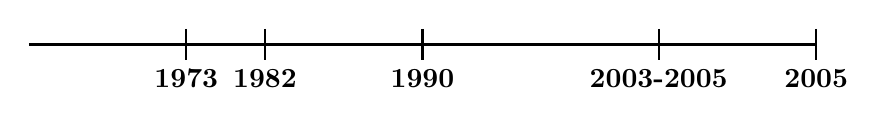
\begin{tikzpicture}[scale=1, every node/.style={scale=1}]
        % Draw timeline line
        \draw[thick] (0,0) -- (10,0);

        % Timeline markers
        \draw[thick] (2,0.2) -- (2,-0.2);
        \draw[thick] (3,0.2) -- (3,-0.2);
        \draw[thick] (5,0.2) -- (5,-0.2);
        \draw[thick] (8,0.2) -- (8,-0.2);
        \draw[thick] (10,0.2) -- (10,-0.2);

        % Years
        \node[below] at (2,-0.2) {\textbf{1973}};
        \node[below] at (3,-0.2) {\textbf{1982}};
        \node[below] at (5,-0.2) {\textbf{1990}};
        \node[below] at (8,-0.2) {\textbf{2003-2005}};
        \node[below] at (10,-0.2) {\textbf{2005}};
    \end{tikzpicture}
}

% \setbeameroption{show notes on second screen=right}
% \setbeameroption{show only notes}
%
\definecolor{backcolour}{rgb}{0.98,0.98,0.95}
\newcommand{\listingsttfamily}{\fontfamily{IBMPlexMono-TLF}\small}

\lstdefinestyle{prettycode}{
  basicstyle=\listingsttfamily,
  backgroundcolor=\color{backcolour},
  aboveskip={0.9\baselineskip},               
  keepspaces=true,
}
\lstset{style=prettycode}


\begin{document}
  \maketitle
  \section{Version Control Systems}
  \begin{frame}{Scenario: A New Project}
    % Imagine you're working on a project and create the new project file.
    %
    % You work on a file for a bit until you're at a point where you have basic function and want to save your progress. 
    %
    % You leave for the weekend and come back after reaching the conclusion that your approach was wrong, and now want to restart. 
    %
    % You continue this cycle for a while, and your code structure looks something like this.
    \only<1-3>{
    \begin{columns}
        \column{0.6\textwidth}
        \begin{itemize}
          \item[]<1-3> Imagine you're working on a project and create the new project file.
          \item[]<2-3> You work on a file for a bit until you're at a point where you have basic function and want to save your progress. 
          \item[]<3-3> You leave for the weekend and come back after reaching the conclusion that your approach was wrong, and now want to restart.
            % \item \pause You continue this cycle for a while, and your code structure looks something like this.
        \end{itemize}
        
        % 360 x 250
        \column{0.4\textwidth}
        \only<1>{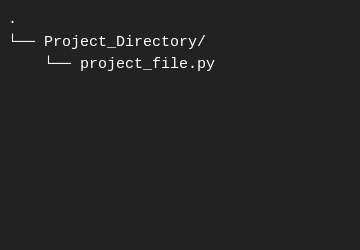
\includegraphics[width=\linewidth]{images/dir_tree_1.png}}
        \only<2>{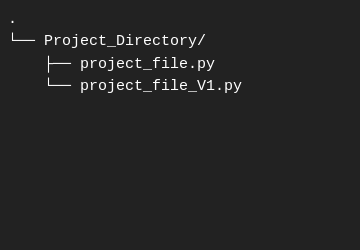
\includegraphics[width=\linewidth]{images/dir_tree_2.png}}
        \only<3>{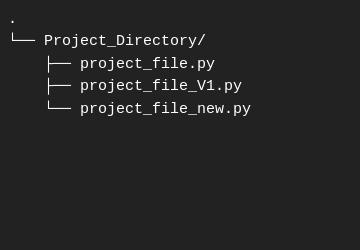
\includegraphics[width=\linewidth]{images/dir_tree_3.png}}
    \end{columns}
  }
    
    \only<4>{\centering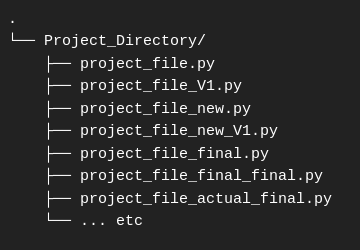
\includegraphics[width=0.7\linewidth]{images/dir_tree_4.png}}
  \end{frame}

  \begin{frame}{What is the Solution?}
  \begin{itemize}
    \item[]<1-> This problem has plagued software development since early on. 
      \item[]<2-> The approach in the scenario asks for a lot of time, effort, and discipline to maintain.
      \item[]<3-> In the case of a collaborative project, it would be difficult to not make clashing changes, and when changes are made, time would need to be spent to manually merge the different versions of files.
      \item[]<4-> There have been efforts to automate this since the 80s.
    \end{itemize}
  \end{frame}


\section{Version Control Systems - A History}

\begin{frame}{Source Code Control System (SCCS)}
  \timeline

  \begin{itemize}
    \item[\textbf{1973}]<1-> A Version control system designed to track source code changes.
    \item[]<2-> Developed at Bell Labs for an IBM System/370.
    \item[]<3-> Was the dominant version control system until later systems, such as RCS and CVS, were released.
  \end{itemize}

  \begin{figure}
    \begin{center}
      
\includegraphics[width=0.75\textwidth]{images/Bell_Laboratories_logo.png}
    \end{center}
    \caption{Bell Laboratories logo (1969 - 1983)}\label{fig:bell_labs}
  \end{figure}
  
  
\end{frame}

%  Frame 1 - RCS
\begin{frame}{Version Control Systems Timeline - RCS}
  \timeline

  \begin{columns}

      \column{0.7\textwidth}
    \begin{itemize}
      \item[\textbf{1982}]<1-> Revision Control System was introduced.
      \item[]<2-> Written by Walter Tichy at Purdue University.
      \item[]<3-> Consisted of a set of UNIX commands that kept track of differences between files known as 'reverse deltas'.
      \item[]<4-> Used a model that locked files when they were being edited, known as a 'pessimistic locking model'. If you also wanted to edit it, you had to wait.
    \end{itemize}

    \column{0.23\textwidth}
    \begin{figure}
      \hfill
      \begin{minipage}{\textwidth}
        \centering
        
\includegraphics[width=\textwidth]{images/Heckert_GNU_white.png}
        \caption{GNU mascot Heckert}
        \label{fig:heckert}
      \end{minipage}
    \end{figure}
    
  \end{columns}
    
  \note[item]{Reverse deltas are the changes needed to be made to get from newer to older versions. Old versions can be reached by sequentially applying these deltas.}
\end{frame}

% Frame 2 - CVS
\begin{frame}{Version Control Systems Timeline - VCS}
    \timeline
  \begin{columns}

      \column{0.75\textwidth}
    \begin{itemize}
      \item[\textbf{1990}]<1-> Concurrent Versions System was introduced, developed by Dick Grune. 
      \item[]<2-> A front end of the RCS, it added repository-level change tracking. 
      \item[]<3-> Included a client-server model, where a server stores the project and its history, and a complete copy can be checked out and later checked in.
      \item[]<4-> Replaced 'pessimistic' model with an 'optimistic' model, meaning multiple people could edit the same file, merging later. 
    \end{itemize}


    \column{0.23\textwidth}
    \begin{figure}
      \hfill
      \begin{minipage}{\textwidth}
        \centering
        
\includegraphics[width=\textwidth]{images/TortoiseCVS_Logo.png}
        \caption{TortoiseCVS mascot, Charlie Vernon Smythe}
        \label{fig:charlie}
      \end{minipage}
    \end{figure}
    
  \end{columns}


\end{frame}

% Frame 3 - DVCS
\begin{frame}{Version Control Systems Timeline - DVCS}
    \timeline
    \begin{columns}
      
      \column{0.75\textwidth}
      \begin{itemize}
        \item[\textbf{2003-2005}]<1-> Distributed Version Control Systems started being introduced. 
        \item[]<2-> A server stores all files and their histories.
        \item[]<3-> When someone asks for the repository, they receive a mirror of this on their local machine. 
        \item[]<4-> Almost all processes occur offline, and are very fast as a result.
      \end{itemize}


    \end{columns}

\end{frame}

\begin{frame}{Distributed Version Control Systems}

  \begin{figure}
    \begin{center}
      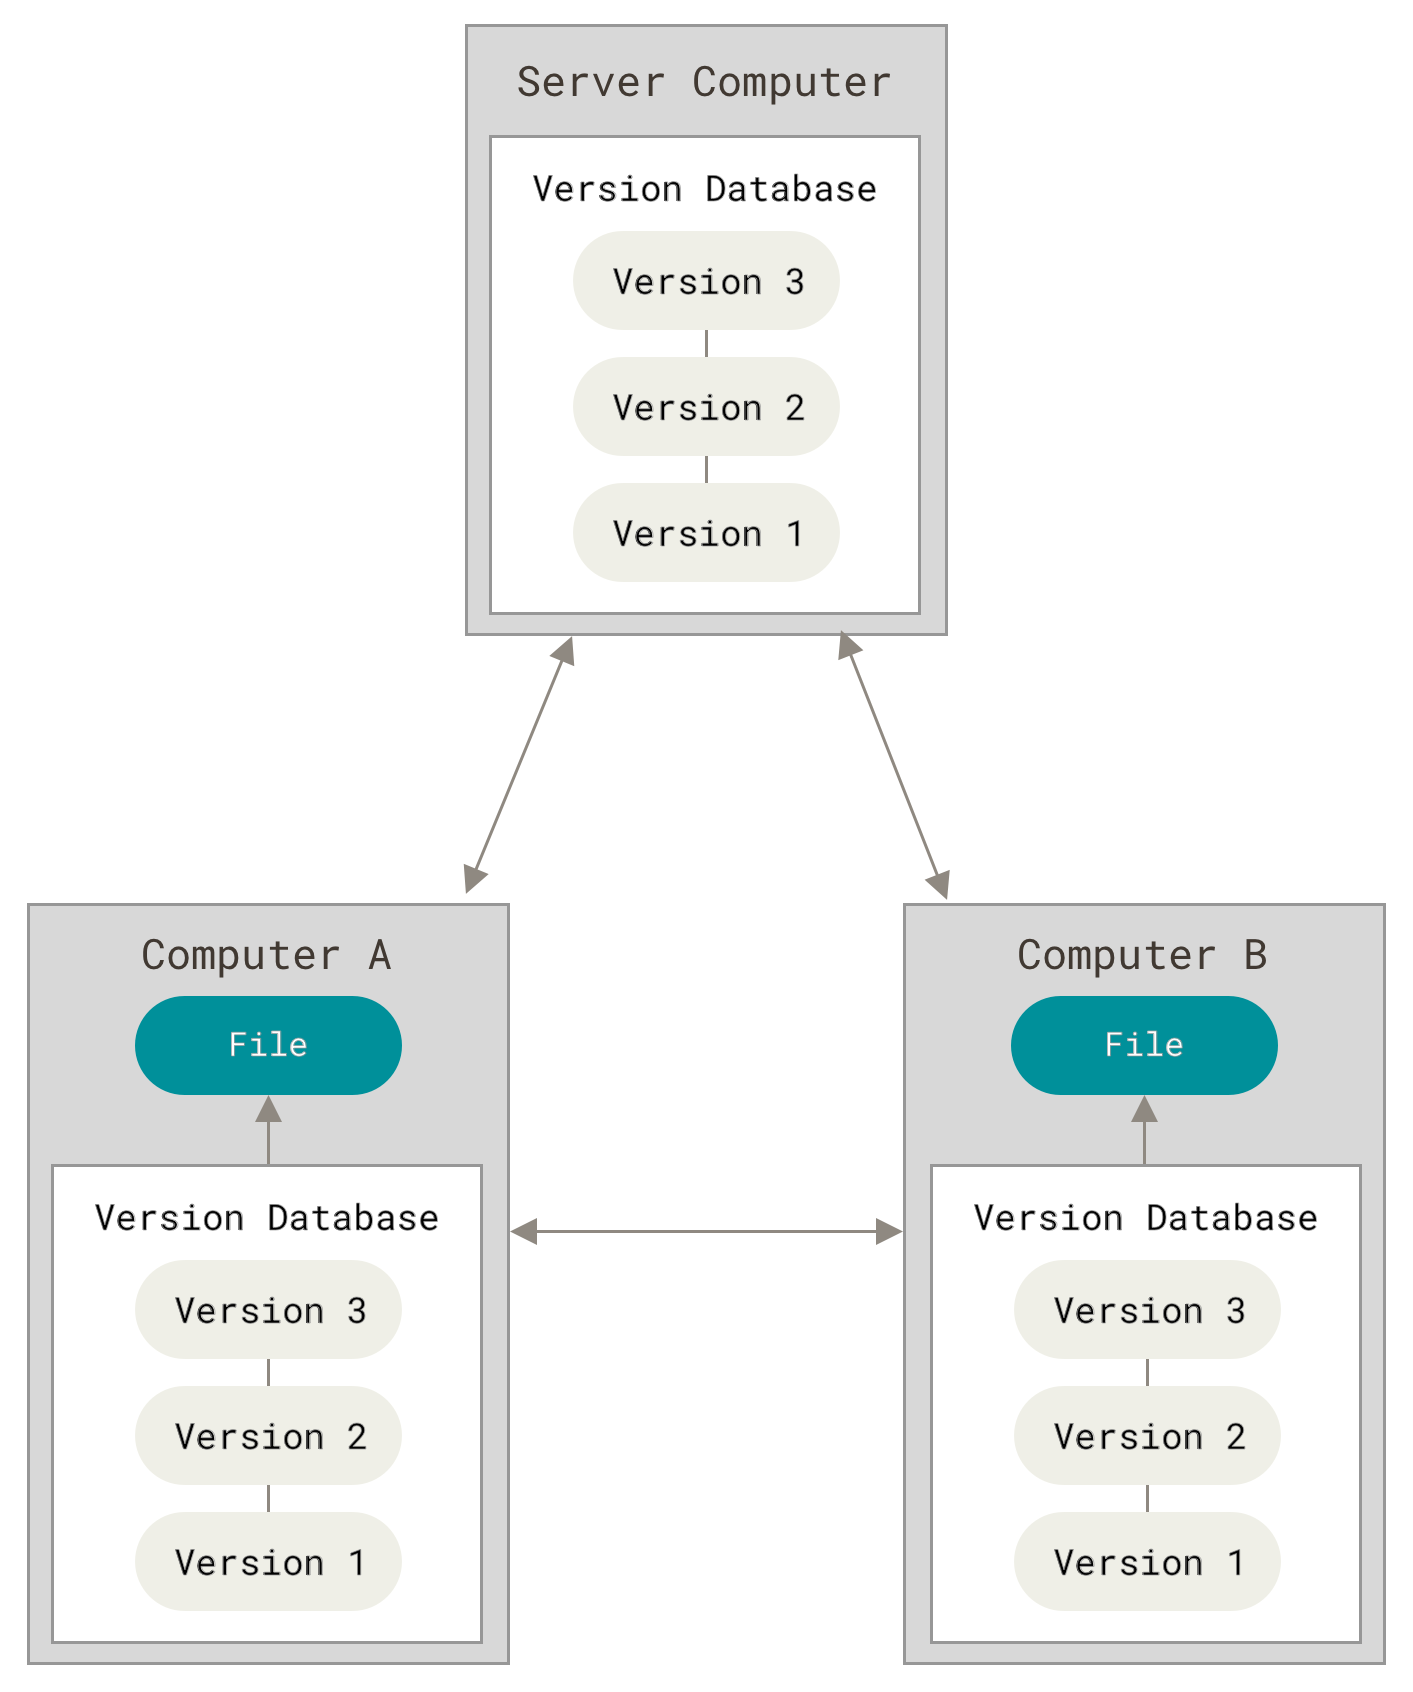
\includegraphics[height=0.95\textheight]{images/DVCS.png}
    \end{center}
    \caption{Outline of DVCS}\label{fig:DVCS_structure}
  \end{figure}
  
  
\end{frame}

% Frame 4 - Git
\begin{frame}{Version Control Systems Timeline - Git}
    \timeline

    \begin{columns}
      \column{0.75\textwidth}
      \begin{itemize}
        \item[\textbf{2005}]<1-> Git is released by Linus Torvalds while developing the Linux Kernel.
        \item[]<2-> Linus started developing Git on \textbf{3rd April 2005} after a disagreement with BitKeeper, a proprietary DVCS.
        \item[]<3-> Goals when developing Git included: \begin{itemize}
          \item Use CVS as an example of what not to do 
          \item Supported a distributed workflow 
          \item Make it safe against corruption
        \end{itemize}
      \item[]<4-> Linus achieved his performance goals on \textbf{29th April 2005}.
      \end{itemize}
      
      \column{0.23\textwidth}
      \begin{figure}
      \hfill
      \begin{minipage}{\textwidth}
        \centering
        
\includegraphics[width=\textwidth]{images/git_logo.png}
        \caption{Logo of git}
        \label{fig:git_logo}
      \end{minipage}
    \end{figure}

    \end{columns}

\end{frame}

\section{Git}

\begin{frame}{So how does git work?}
  \begin{columns}
    \column{0.75\textwidth}
    \begin{itemize}
      \item <1-4> Git is a DVCS, so each developer has a mirror of the main repository. 
      \item <2-4> The main repository contains a the histories of all its files, which can be accessed by anyone with the repository.
      \item <3-4> Files are initially untracked, and git needs to be told by the user to track the file.
      \item <4-4> Files have a 'life cycle' in git.
    \end{itemize}
  \end{columns}

\end{frame}

\begin{frame}{Git Life Cycle}
    \begin{figure}
      \hfill
        \centering
        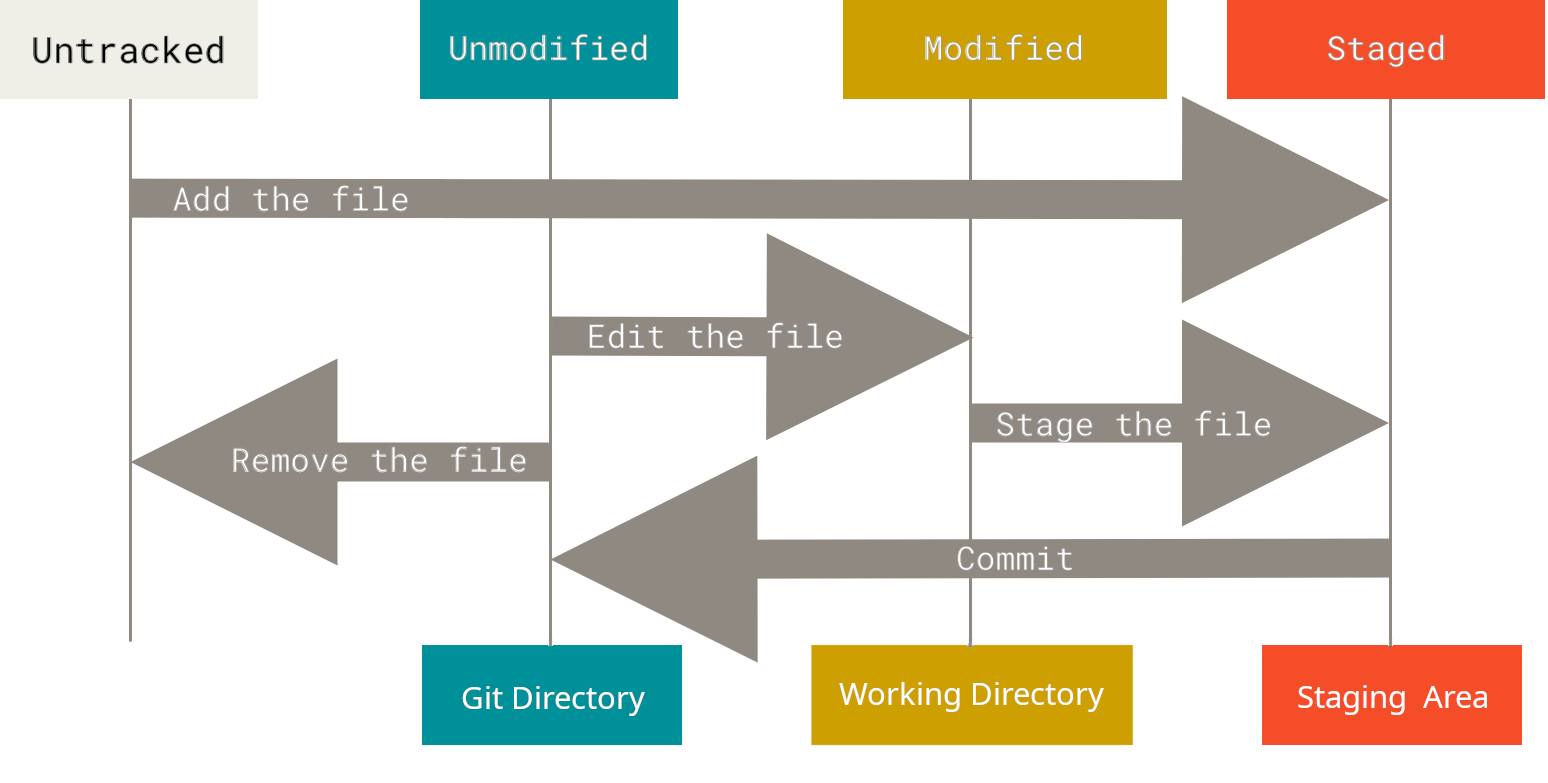
\includegraphics[width=\textwidth]{images/git_lifecycle.png}
        \caption{Life cycle of a file in a git repository}
        \label{fig:git_lifecycle}
    \end{figure}

    \note[item]{Files exist in three different stages in a git directory, Working directory, staging area, and git directory.}
    \note[item]{Working directory: git is aware of the files, but isn't tracking them yet.}
    \note[item]{Staging area: files in the working directory can be selected to be tracked by git by adding them to the staging area.}
    \note[item]{Git directory: files that have been added to the staging area can now be committed to the git directory, taking a snapshot of the files. When committing, a message briefly explaining the commit is included, as well as the author and time of the commit.}

\end{frame}

\begin{frame}{Using git}
  \begin{itemize}
    \item<1-> Git is a command line tool, and is normally used directly from the terminal.
    \item<2-> There are GUI clients for git, but for smaller projects these don't offer many useful features. 
    \item<3-> For basic use, only a handful of commands are needed.
    \item<4-> Git is an open source software, and can be installed easily via many package managers. 
  \end{itemize}

\end{frame}

\begin{frame}[fragile]{Using git - Config}

    \begin{itemize}
      \item <1-> Since git keeps track of the author of each commit, each machine has an associated user name and user email 
      \item <2-> Only needs to be set once.
    \end{itemize}
    \begin{onlyenv}<3>
    \begin{lstlisting}[frame=single]
      git config --global user.name ``<NAME>"
      git config --global user.email <EMAIL>
    \end{lstlisting}
  \end{onlyenv}

\end{frame}

\begin{frame}[fragile]{Using git - Initialising a git repository}
 \begin{itemize}
    \item <1-> A git repository can be initialised in any directory. 
      \item<2-> Initialising the directory adds a \lstinline{.git} folder, which is the git directory.
  \end{itemize} 
  \begin{onlyenv}<3->
    \begin{lstlisting}[frame=single]
      git init <DIR>
    \end{lstlisting}
  \end{onlyenv}
\end{frame}

\begin{frame}[fragile]{Using git - Staging files}
  \begin{itemize}
    \item <1-> From the git life cycle before, we know that files are staged when we want git to track them.
    \item <2-> These can be new files, or files that have been edited and are in a modified stage. 
    \item <3-> Moves files from the working directory to the staging area.
    \item <4-> the flag of \lstinline{--a} or \lstinline{-all} can be added to stage all files. This can be bad as we should not track files that are dynamic, i.e. log files, result files, config files, etc.
  \end{itemize}  
  \begin{onlyenv}<4->
    \begin{lstlisting}[frame=single]
      git add [<files>][-A]
    \end{lstlisting}
  \end{onlyenv}
\end{frame}

\begin{frame}[fragile]{Using git - Commiting files to git directory}
  \begin{itemize}
    \item <1-> Now that the files are staged, they can be committed to the git directory.
    \item <2-> This will take a snapshot of the file. 
    \item <3-> Information related to the commit is also stored in the git directory, i.e. name of files, date and time, author, and commit message.
    \item <4-> You need to include a commit message when commiting. Can be done in the command line as shown, or in the default text editor if \lstinline{-m `<MESSAGE>'} is not included.
  \end{itemize}
  \begin{onlyenv}<4->
    \begin{lstlisting}[frame=single]
      git commit -m `<COMMIT MESSAGE>'
    \end{lstlisting}
  \end{onlyenv}
\end{frame}

\begin{frame}{Using git - GitHub}
  \begin{itemize}
    \item <1-> So far, only the life cycle of git has been explored. To have a remote repository, a server to host the repo is needed.
    \item <2-> GitHub is a common choice, although there are alternatives.
    \item <3-> A local repository can be pushed to a remote repository to upload the commits from the local git repo.
    \item <4-> \textbf{Everything mentioned previously has been local. A remote repository is not needed for version control. }
  \end{itemize}
\end{frame}

\begin{frame}{Git - Other Concepts}
  \begin{itemize}
    \item[] <1-> Branching: Allows for a seperate environment where changes can be made without risking the codebase. Can be merged with the main branch to implement changes.
  \end{itemize}
  \begin{figure}
    \begin{center}
      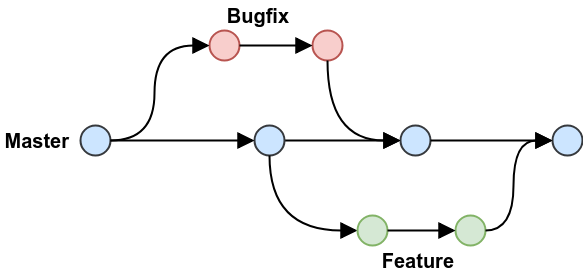
\includegraphics[width=0.7\textwidth]{images/branching.png}
    \end{center}
    \caption{Branching of git repository.}\label{fig:branching}
  \end{figure}
  
\end{frame}

\begin{frame}{Git - Other Concepts}
  \begin{itemize}
    \item<1-> Merging: When combining two branches/forks, \lstinline{git merge} checks for conflicts and lets the user device how to resolve these. 
    \item<2-> Log and History: Can check the commit history with \lstinline{git log} and see file changes with \lstinline{git diff}
    \item <3-> Revert: To revert to a previous commit, \lstinline{git revert} creates a new commit that undose the previous commit.
      \item<4-> Stashing: This command saves the state of the working directory, but reverts to the last commmit. Used as a way of getting a clean directory. 
  \end{itemize}
\end{frame}

\begin{frame}[fragile]{Using Git - Summary}
  \begin{itemize}
    \item[]<1-1> What commands do I need?
    \item[]<2-> To get basic functionality from git, commands to maintain the basic git life cycle are only needed. Generally, remember to following:

  \end{itemize}
  \begin{onlyenv}<3->
    \begin{lstlisting}[frame=single]
      git add <files>
      git commit -m "<COMMIT MESSAGE>"
      git push
    \end{lstlisting}
  \end{onlyenv}
\end{frame}

\begin{frame}{Useful Resources}
Git and GitHub are commonly used tools, and so there is a lot of good resources to use. \pause 


  \begin{itemize}
    \item <2-> The git documentation includes guides (https://git-scm.com/)
    \item <3-> \textbf{Oh Shit, Git!?} inludes fixes to common problems (https://ohshitgit.com/)
    \item <4-> \textbf{Learn Git Branching} is an interactive tool to learn git (https://learngitbranching.js.org/)
  \end{itemize}
\end{frame}

\end{document}
